
\begin{figure}[h]
    \centering
    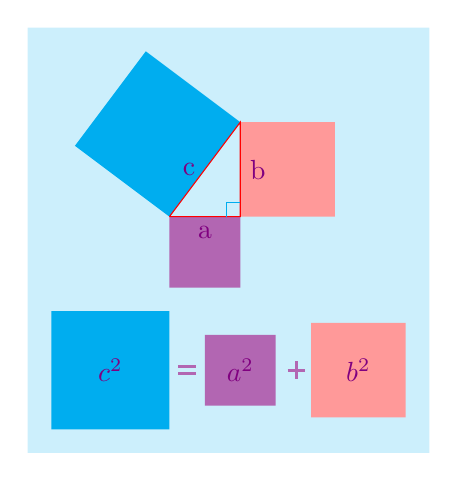
\begin{tikzpicture}[scale=0.3]
        %\draw [ultra thick, help lines] (-10,-10) grid (10,10);
        %\draw [line width=2pt, rounded corners, fill=red] (0,0) rectangle (3,5);
        \path [fill=cyan!20] (-9,-10) -- (-9,8) -- (8,8) -- (8,-10) -- (-9,-10);
        \path [fill=cyan] (-3,0) -- (0,4) -- (-4,7) -- (-7,3) -- (-3,0);
        \path [fill=red!40] (0,4) -- (4,4) -- (4,0) -- (0,0) -- (0,4);
        \path [fill=violet!60] (-3,0) -- (-3,-3) -- (0,-3) -- (0,0) -- (-3,0);
        \draw[red, line width=0.4pt] (-3,0) -- (0,4) -- (0,0) -- (-3,0);
        \draw[cyan, thin] (-0.6,0) -- (-0.6,0.6) -- (0,0.6) ;
        \node [below, violet] at (-1.5,0) {a};
        \node [right, violet] at (0,2) {b};
        \node [left, violet] at (-1.5,2) {c};
        
        \path [fill=cyan] (-8,-9) -- (-8,-4) -- (-3,-4) -- (-3,-9) -- (-8,-9);
        \node [violet] at (-5.5,-6.5) {$c^2$};
        \path [fill=violet!60] (-1.5,-8) -- (-1.5,-5) -- (1.5,-5) -- (1.5,-8) -- (-1.5,-8);
        \node [violet] at (0,-6.5) {$a^2$};
        \path [fill=red!40] (3,-4.5) -- (7,-4.5) -- (7,-8.5) -- (3,-8.5) -- (3,-4.5);
        \node [violet] at (5,-6.5) {$b^2$};
        
        \draw[violet!60, line width=1pt] (-1.875,-6.35) -- (-2.625,-6.35);
        \draw[violet!60, line width=1pt] (-1.875,-6.65) -- (-2.625,-6.65);
        
        \draw[violet!60, line width=1pt] (2,-6.5) -- (2.75,-6.5);
        \draw[violet!60, line width=1pt] (2.375,-6.125) -- (2.375,-6.875);
        
    \end{tikzpicture}
    \caption{Visual representation of the famous Pythagorean theorem.}
    \label{fig:pythagorean theorem}
\end{figure}
